\documentclass{report}
\usepackage[a4paper, portrait, margin=0.4in,bottom=0.7in]{geometry}
\usepackage{graphicx,wrapfig,amsmath,amssymb,algorithm,algpseudocode,caption,subcaption,hyperref,enumitem,tikz,mathabx,amsthm} 

\newtheorem{theorem}{Theorem}[section]
\newtheorem{corollary}{Corollary}[theorem]
\newtheorem{lemma}[theorem]{Lemma}
\usepackage{mathtools}

\title{Automata Theory}
\author{Abhijit Amrendra Kumar}
\date{August 2023}

\setlength\parindent{0pt}
\newcommand{\Dhat}{\hat{\Delta}}
\newcommand{\dhat}{\hat{\delta}}
\newcommand{\hr}{\hrule\vspace{4mm}}

\begin{document}

\maketitle

\chapter{Introduction}
\section{Abstract}

Automata theory involves the study of systems of computations.
\begin{itemize}[leftmargin=0.2in]
  \item (formal verification) What are the properties of a concrete algorithm given in a system of computation? What methods can be used to analyse such questions?
  \item (expressivity) What kind of calculations are possible in a system of computation? Can system A compute everything that is computable in system B?
  \item (computability) Is a problem solvable in given system of computation?
\end{itemize}

Some larger questions include
\begin{itemize}[leftmargin=0.2in]
  \item Is there a most powerful system of mechanical computation ?
  \item Are there problems which cannot be mechanically solved ?
\end{itemize}

\section{Course Syllabus}
\begin{itemize}[leftmargin=0.2in]
  \item \textbf{Finite State Automata}
        \begin{itemize}[leftmargin=0.2in]
          \item Deterministic Finite Automata (DFA) and its uses.
          \item DFA, NFA and Equivalence
          \item Closure Properties and Decision Problems
          \item Regular Expressions and Equivalence to DFA
          \item Homomorphisms
          \item DFA minization
          \item Pumping Lemma
          \item Myhill Nerode Theorem
        \end{itemize}
  \item \textbf{Pushdown Automata and Context-Free Languages}
        \begin{itemize}[leftmargin=0.2in]
          \item Phrase structured Grammars and Chomsky Hiearchy
          \item Context Free Grammars (CFG), Uses of CFG, Normal forms
          \item Push Down Automata (PDA)
          \item Equivalence of CFG and PDA
        \end{itemize}
  \item \textbf{Turing Machines and Computability}
        \begin{itemize}[leftmargin=0.2in]
          \item Definition and Examples of Turing Machines
          \item Robustness (Multihead TM, Nondeterministic TM)
          \item Universal Turing Machines
          \item Halting Problem and Undecidability
          \item Variety of Unsolvable Problems
          \item Many-to-One reductions
          \item Rice Theorem
        \end{itemize}
\end{itemize}

\section{References}
\begin{itemize}
  \item \href{https://cse.iitb.ac.in/~pandya58/CS310/automata.html}{Course Webpage}
  \item Dexter Kozen, Automata and Computability. Springer, 1997.
  \item Hopcroft, Motwani, Ullman, Introduction to Automata Theory, Languages and Computation, PearsonEducation Asia, 2006.
\end{itemize}

% ----------------------------------------------------------------

\chapter{Words and Languages, Deterministic Finite Automata}

\section{Decision Problems and Automata}

A decision problem is a problem which has \verb|yes| or \verb|no| as answer.

\subsection{What is an Automaton ?}

Consider a set of input instances \verb|A| and a subset \verb|B| of \verb|A| which only contains instances for which the answer is \verb|yes|. An \textbf{automaton} for $(A,B)$ is a machine which can solve any given instance $x \in A$ of the decision problem: given $x \in A$, determine whether $x \in B$.

\subsection{Problem Instances as Strings}

To give input to an automaton, we will use strings of symbols.
\begin{itemize}[leftmargin=0.2in]
  \item Alphabet $\Sigma$: A finite set of symbols/letters.
        \begin{itemize}
          \item Ex. $\Sigma = \{0,1\}$
          \item We will use $a,b,c,...$ to denote letters.
        \end{itemize}
  \item Word over an alphabet $\Sigma$ is a finite sequence of symbols from $\Sigma$.
        \begin{itemize}[leftmargin=0.2in]
          \item Ex. $01001$
          \item We will use $x,y,z,...$ to denote words.
        \end{itemize}
  \item $\Sigma^*$ denotes the set of all words over the alphabet $\Sigma$.
  \item $\epsilon$ denotes the empty word.
  \item $|x|$ denotes the length of word $x$.
        \begin{itemize}[leftmargin=0.2in]
          \item Ex. $|101101| = 6$
          \item $|\epsilon| = 0$
        \end{itemize}
  \item Catenation of 2 words $x,y$ is denoted by $x \cdot y$.
        \begin{itemize}[leftmargin=0.2in]
          \item Ex. $ab \cdot abba = ababba$
          \item $|x \cdot y| = |x| + |y|$
          \item $x\cdot (y \cdot z) = (x \cdot y) \cdot z$
          \item $\epsilon \cdot x = x \cdot \epsilon = x$
          \item $x^{n+1} = (x^n) \cdot x$
        \end{itemize}
\end{itemize}

\section{Language}

A \textbf{Language} over an alphabet $\Sigma$ is any subset of $\Sigma^*$.

\begin{itemize}[leftmargin=0.2in]
  \item We use $A,B,C,...$ to denote languages
  \item We use $\#a(x)$ to denote the count of $a$ in $x$
\end{itemize}

\begin{itemize}[leftmargin=0.2in]
  \item Here are some examples
        \begin{itemize}[leftmargin=0.2in]
          \item $A = \{ a^p \ | \ p \text{ is a prime} \}$
          \item $A = \{ x \in \{0,1\}^* \ | \ \#0(x) = \#1(x) \}$
          \item $A = \{ x \in \{0,1\}^* \ | \ \exists i \in \mathbb{N}, \ x\text{ is the binary representation of } 2^i \}$
        \end{itemize}
\end{itemize}

\subsection{Operations on Languages}

Let $A,B$ be languages over an alphabet $\Sigma$.
\begin{itemize}[leftmargin=0.2in]
  \item $A \cup B = \{ x \in \Sigma^* \ | \ x \in A \text{ or } x \in B \}$
  \item $A \cap B = \{ x \in \Sigma^* \ | \ x \in A \text{ and } x \in B \}$
  \item $\sim A = \{ x \in \Sigma^* \ | \ x \notin B \}$
  \item $A \cdot B = \{ x \cdot y \ | \ x \in A \text{ and } y \in B \}$
        \begin{itemize}[leftmargin=0.2in]
          \item Ex. $A = \{a,ab\}, B = \{b,ba\} \implies A \cdot B = \{ ab,aba,abb,abba \}$
        \end{itemize}
\end{itemize}

\begin{itemize}[leftmargin=0.2in]
  \item \textbf{Language Recognition Problem}: Given an input word $x$, determine whether $x \in A$.
  \item All computational problems can be encoded into language recognition problems
  \item Each automaton defines a language
\end{itemize}

\section{Deterministic Finite Automata}

A DFA is given by $Q,\Sigma,\delta,q_0,F$, where
\begin{itemize}
  \item $Q$ is the set of states
  \item $\Sigma$ is the set of alphabets
  \item $\delta: Q \times \Sigma \rightarrow Q$ is the transition function
  \item $q_0 \in Q$ is the initial state
  \item $F \subseteq Q$ is the set of final states
\end{itemize}

A DFA can also be represented by either a transition table, or via a transition diagram.

% DIAGRAM
\begin{itemize}
  \item A run of DFA $A$ on $x = a_0,a_1,...,a_{n-1}$ is a sequence of states $q_0,q_1,...q_n$ s.t $q_i \overset{a_i}{\rightarrow} q_{i+1}$ for $0 \leq i < n$.
  \item For a given word $x$, DFAs have unique runs.
  \item A run is accepting if last state $q_n \in F$
  \item A word is accepted by an automaton if it's run is accepting
\end{itemize}

Language accepted by an automaton $A$ can also be defined as
$$
  L(A) = \{ u \in \Sigma^* | \text{ The run of A on u is accepting } \}
$$
A language is called \textbf{regular} if it is accepted by some DFA.

\subsection{Big Step Semantics}

Given DFA with transition function $\delta: Q \times \Sigma \rightarrow Q$, we can define an extended transition function
$$
  \hat{\delta}: Q \times \Sigma^* \rightarrow Q
$$

Here, $\hat{\delta}(q,x)$ gives the last state of the run of A on word $x$ starting from state $q$. It can be defined inductively as follows
\begin{align*}
  \hat{\delta}(q,\epsilon) & = q,                           \\
  \hat{\delta}(q,ua)       & = \delta(\hat{\delta}(q,u),a), \\
\end{align*}

A word $x$ is accepted by an automaton $A$ iff $\hat{\delta}(q_0,x) \in F$ \\

\textbf{Theorem}: $$\hat{\delta}(q,xy) = \hat{\delta}(\hat{\delta(q,x)},y)$$

\textbf{Proof}:

\section{Constructions on Automata}


% ----------------------------------------------------------------

\chapter{Regular Expressions}
\section{Automata to RegExp}

\textbf{Theorem}:

For every NFA $A = (Q,\Sigma,\Delta,I,F)$, we can construct a language equivalent regular expression $reg(A)$ \\

\textbf{Proof}: \\

\textbf{Construction}:

Define regular expression $\alpha_{p,q}^{X}$ for $X \subseteq Q, \quad p,q \in Q$. This set of words $w$ such that $A$ has a run on $w$ from $p$ to $q$, where all the intermediate states are from $X$. \\

\textbf{Examples}:
$$
  \alpha_{p,q}^{r} = 1 \cdot 0 \qquad \qquad \qquad \alpha_{p,r}^{p,q} = 0^* \cdot 1 \cdot 0
$$

Let's try to compute $\alpha_{p,p}^{p,q,r}$. \\

$\alpha_{p,r}^X$ can be recursively

% ----------------------------------------------------------------

\chapter{Minimizing DFA}

\begin{center}
  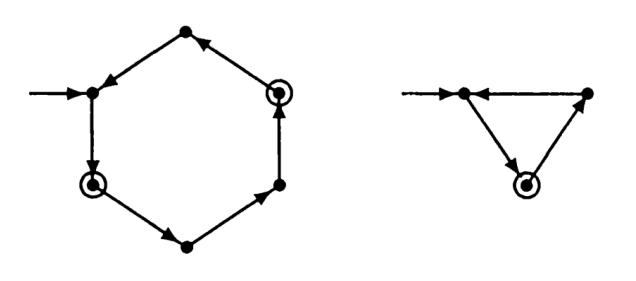
\includegraphics[scale=0.5]{images/mul_dfa.png}
\end{center}

There can be multiple DFAs recognizing the same language. Hence the question arises as to if there exists a minimum DFA which can recognize the same language, and if so, how to find it. \\
We already know that $\epsilon$-NFA to DFA conversion often gives rise to large automaton which are not guaranteed to be optimal in size. The same is true when converting regular expressions to DFA. \\

Let's consider some examples to notice some patterns.

\begin{center}
  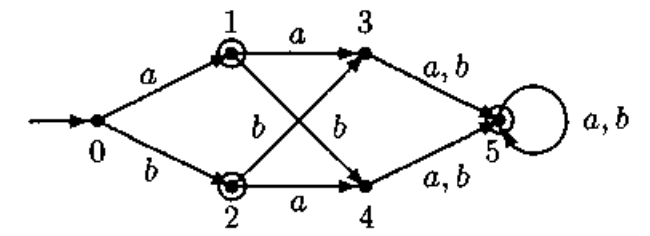
\includegraphics[scale=0.5]{images/large-auto-1.png}
\end{center}

Here's the minimal DFA for the language defined by the above DFA.

\begin{center}
  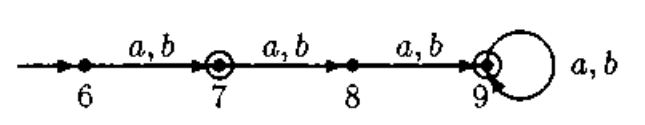
\includegraphics[scale=0.5]{images/minimised-auto-1.png}
\end{center}

The minimization procedure consists of 2 stages:
\begin{itemize}
  \item Get rid of inaccessible states; that is, states q for which there exists no string $x \in \Sigma^*$ such that $\dhat(s,x) = q$
  \item Collapse equivalent states
\end{itemize}

To minimise a DFA, let's first define the following: \\\\

{\Large Equivalent States in a DFA} \\

Two states $p,q$ in an DFA are said to be equivalent states (denoted by $p\approx q$) if
$$ p\approx q \ \overset{\text{def}}{=} \ \forall x \in \Sigma^* (\hat{\delta}(p,x) \in F \iff \hat{\delta}(q,x) \in F)$$

The proposition $\approx$ is an equivalence relation
\begin{itemize}
  \item $\forall p, \ p \approx p$
  \item $\forall p,q, \ p \approx q \implies q \approx p $
  \item $\forall p,q,r, \ p \approx q \land q \approx r \implies p \approx r$
\end{itemize}

It partitions $Q$ into equivalence classes. Let $[p]$ denote the equivalence classes of $p$. \\

\newpage

{\Large Quotient Automaton} \\

% ----------------------------------------------------------------

Given DFA $M=\left(Q, \Sigma, \delta,\left[q_0\right], F\right)$ and $\approx$ as before, the Quotient automaton is $M / \approx \stackrel{\text { def }}{=}\left(Q^{\prime}, \Sigma, \delta^{\prime},\left[q_0\right], F^{\prime}\right)$, where
$$
  \begin{aligned}
    Q^{\prime}              & = \{[p] \mid p \in Q\} \\
    \delta^{\prime}([p], a) & = [\delta(p, a)]       \\
    F^{\prime}              & = \{[f] \mid f \in F\}
  \end{aligned}
$$

\textbf{Lemma}: $\quad p \approx q \implies \forall a \in \Sigma . \quad \delta(p, a) \approx \delta(q, a)$ \\
\textbf{Proof}: \\
Suppose $p \approx q$. Let $a \in \Sigma$, and $y \in \Sigma^*$
\begin{align*}
  \dhat(\delta(p,a),y) \in F & \iff \dhat(p,ay) \in F          \\
                             & \iff \dhat(q,ay) \in F          \\
                             & \iff \dhat(\delta(q,a),y) \in F
\end{align*}

Since $y$ was arbitrary, $\delta(p,a) \approx \delta(q,a)$ by definition of $\approx$. \\

\hr

\textbf{Lemma}: $\quad p \in F \Leftrightarrow [p] \in F^{\prime}$ \\
\textbf{Proof}: \\
LHS implies RHS is evident by definition. For proving that RHS implies LHS, we need to show that if $p \approx q$ and $p \in F$, then $q \in F$. In other words, every equivalence class is either a subset of F, or disjoint from F. This follows by taking $x = \epsilon$ in the definition of $p \approx q$. \\

\hr

\textbf{Lemma}: $\quad \forall \ x \in \Sigma^*, \hat{\delta}^{\prime}([p], x)=[\hat{\delta}(p, x)]$. \\
\textbf{Proof}: By induction on $|x|$ \\
Basis: For $x = \epsilon$,
\begin{align*}
  \dhat'([p],\epsilon) & = [p]                 \\
                       & = [\dhat(p,\epsilon)]
\end{align*}

Induction step: Assume $\dhat'([p],x) = [\dhat(p,x)]$ and let $a \in \Sigma$
\begin{align*}
  \dhat'([p],xa) & = \delta'(\dhat'([p],x),a) \\
                 & = \delta'([\dhat(p,x)],a)  \\
                 & = [\delta(\dhat(p,x),a)]   \\
                 & = [\dhat(p,xa)]            \\
\end{align*}

\hr

\textbf{Theorem}: $L(M/\approx) = L(M)$ \\
\textbf{Proof}:
\begin{align*}
  x \in L(M/\approx) & \iff \dhat'([q_0],x) \in F' \\
                     & \iff [\dhat(q_0,x)] \in F'  \\
                     & \iff \dhat(q_0,x) \in F     \\
                     & \iff x \in L(M)
\end{align*}

\hr

{\Large $M/\approx$ cannot be collapsed further} \\

It is conceivable that after doing the quotient construction once, we might be able to collapse even further by doing it again. It turns out that once is enough. To see this, let's do the quotient construction a second time. \\
Define \\
$$
  [p] \sim [q] \overset{\text{def}}{\iff} \forall \ x \in \Sigma^* (\dhat'([p],x) \in F' \iff \dhat'([q],x) \in F')
$$
This is exactly the same definition as $\approx$ above, only that it is applied to $M/\approx$. Now:
\begin{align*}
  [p] \sim [q] & \implies \forall \ x \in \Sigma^* (\dhat'([p],x) \in F' \iff \dhat'([q],x) \in F') \\
               & \implies \forall \ x \in \Sigma^* ([\dhat(p,x)] \in F' \iff [\dhat(q,x)] \in F')   \\
               & \implies \forall \ x \in \Sigma^* (\dhat(p,x) \in F \iff \dhat(q,x) \in F)         \\
               & \implies p \approx q                                                               \\
               & \implies [p] = [q]
\end{align*}

\hr

{\Large Minimization algorithm}

\begin{itemize}
  \item Make pairs table with $(p, q) \in Q \times Q$ and $p \leq q$.
  \item Mark $(p, q)$ if $p \in F \wedge q \notin F$ or vice versa.
  \item Repeat following steps until no change occurs.
        \begin{itemize}
          \item Pick each unmarked state $(p, q)$.
          \item If $(\delta(p, a), \delta(q, a))$ is marked for some $a \in \Sigma$ then mark $(p, q)$.
        \end{itemize}
  \item For each pair, $p \approx q$ iff $(p, q)$ is unmarked.
\end{itemize}
\textbf{Termination}: In each pass at least one new pair must get marked. \\

\textbf{Theorem}: $(p, q)$ is marked iff $\exists x \in \Sigma^*$, $\dhat(p, x) \in F \wedge \dhat(q, x) \notin F$ or vice versa iff $p \not \approx q$ \\
\textbf{Proof}: \\
Base \\

% TODO

\hr

A nice way to look at the automaton is as a finite automaton itself. Let
$$
  Q =\{ \{p,q\} | p,q \in Q, p \neq q \}
$$

Define a non-deterministic transition function $\Delta: Q \rightarrow 2^Q$ on $Q$ as follows:
$$
  \Delta(\{p,q\},a) = \{ \{ p',q' \} | p = \delta(p',a), q = \delta(q',a) \}
$$

Define a set of start states $S \subseteq Q$ as follows:
$$
  S = \{ \{p,q\} | p \in F, q \notin F \}
$$

Step 2 of the algorithm marks the elements in $S$, and step 3 marks the pairs in $\Delta(\{p,q\},a)$ when $\{p,q\}$ is marked for any $a \in \Sigma$. In these terms, the above theorem says that $p \not\approx q$ if $\{p,q\}$ is accessible in this automaton.

% ----------------------------------------------------------------

\chapter{Myhill-Nerode Relations}

\section{Introduction}

Two DFAs $M = (Q_M,\Sigma,\delta_M,s_M,F_M), N = (Q_N,\Sigma,\delta_N,s_N,F_N)$ are said to be \textbf{isomorphic} if there is a bijection $f: Q_M \rightarrow Q_N$ such that
\begin{itemize}
  \item $f(s_M) = s_N$
  \item $f(\delta_M(p,a)) = \delta_N(f(p),a) \forall \ p \in Q_M, a \in \Sigma$
  \item $p \in F_M \iff f(p) \in F_N$
\end{itemize}

In other words, they are essentially the same automaton, but with different names for their states.

\section{Definition}

Let $\equiv$ be an equivalence relation over $\Sigma^*$.
\begin{itemize}
  \item $\equiv$ is right congruent if $\forall x, y \in \Sigma^*, a \in \Sigma$ we have
        $$
          x \equiv y \quad \Rightarrow \quad x \cdot a \equiv y \cdot a
        $$
  \item Let $R \subseteq \Sigma^*$ (not necessarily regular). $\equiv$ refines $R$ if $\forall x, y \in \Sigma^*$
        $$
          x \equiv y \quad \Rightarrow \quad(x \in R \Leftrightarrow y \in R)
        $$
  \item $\equiv$ is of finite index if $\equiv$ partitions the $\Sigma^*$ into only finitely many equivalence classes.
  \item Equivalence relation $\equiv$ is called Myhill-Nerode Relation refining $R$ if it satisfies all the three properties above.
  \item $\equiv$ is called Weak Myhill Nerode relation Refining $R$ if it satisifies the first two properties.
\end{itemize}

\section{Machine Equivalence}

Given a DFA $A = (Q,\Sigma,\delta,q_0,F)$, define the induced equivalence $\equiv_A$ over $\Sigma^*$ as follows:
$$
  x \equiv_A y \overset{\text{def}}{=} \dhat(q_0,x) = \dhat(q_0,y)
$$

Proposition $\equiv_A$ is a Myhill-Nerode relation refinning $L(A)$.

Proof Method: Check the following
\begin{itemize}
  \item $\equiv_A$ is an equivalence relation for $\Sigma^*$
  \item $x\equiv_A y \implies \forall \ a, xa \equiv_A ya$
  \item $x\equiv_A y \implies (x \in L(A) \iff y \in L(A))$
  \item $\equiv_A$ is of finite index
\end{itemize}

\section{From Equivalence to DFA}

Let $\equiv_A$ be Myhill-Nerode refining $R$. Define DFA $A_{\equiv} \overset{\text{def}}{=} (Q,\Sigma,\delta,S,F)$ as follows:
\begin{align*}
  Q             & \overset{\text{def}}{=} \{ [x] \ | \ x \in \Sigma^* \} \\
  q_0           & \overset{\text{def}}{=} [\epsilon]                     \\
  F             & \overset{\text{def}}{=} \{ [x] \ | \ x \in R \}        \\
  \delta([x],a) & \overset{\text{def}}{=} [xa]
\end{align*}

\begin{theorem}
  $L(A_{\equiv}) = R$
\end{theorem}
\begin{proof}
  \begin{align*}
    x \in L(A_{\equiv}) & \iff \dhat([\epsilon],x) \in F \\
                        & \iff [\epsilon x] \in F        \\
                        & \iff x \in R
  \end{align*}
\end{proof}

\begin{lemma}
  $\dhat([x],y) = [xy]$
\end{lemma}
\begin{proof}
  Induction on $y$

  {\color{blue} Base step}
  $$
    \dhat([x],\epsilon) = [x] = [x\epsilon]
  $$

  {\color{blue} Induction step}
  \vspace{1mm}

  Assuming the lemma holds for $y$,
  \begin{align*}
    \dhat([x],ya) & = \delta(\dhat([x],y),a) \\
                  & = \delta([xy],a)         \\
                  & = [xya]
  \end{align*}
\end{proof}

\section{Correspondence}

The $\equiv_A$ and $A_{\equiv}$ are inverses of each other.

\begin{theorem}
  $\equiv_{A_\equiv} = \ \equiv$
\end{theorem}

\begin{theorem}
  If $A$ is an automaton without unreachable states, then $A_{\equiv}$ is isomorphic to $A$
\end{theorem}

\section{Refining Equivalences}


\end{document}